\documentclass[50pt]{article}
\RequirePackage{pdfpages}
\renewcommand{\baselinestretch}{1.4}
\RequirePackage{amsthm,amssymb,amsmath,graphicx}
\RequirePackage{color}
\RequirePackage[top=2cm, bottom=2cm, left=2.5cm, right=3cm]{geometry}
\RequirePackage[pagebackref=false,colorlinks,linkcolor=blue,citecolor=magenta]{hyperref}
\RequirePackage{xepersian}
\RequirePackage{MnSymbol}
\RequirePackage{graphicx}
\newcommand{\wid}{1.8in}
\newtheorem{theorem}{Theorem}
\newcommand{\hl}{
\begin{center}
\line(1,0){450}
\end{center}}
\newenvironment{amatrix}[1]{%
\left[\begin{array}{@{}*{#1}{c}|c@{}}
}{%
\end{array}\right]
}
\settextfont{B Nazanin}
\setlatintextfont{Times New Roman}

\begin{document}
\setLTR 




\begin{RTL}
\Large{








\begin{center}
به نام خدا

سوالات پیشنهادی میان ترم
\end{center}
\hl
سوال 1) (سوال 20 از فصل 1 کتاب اوپنهایم) یک سیستم خطی، دارای جفت ورودی-خروجی های زیر است:
$$
x(t)=e^{j2t}\overset{S}{\Longrightarrow}y(t)=e^{j3t}
$$
$$
x(t)=e^{-j2t}\overset{S}{\Longrightarrow}y(t)=e^{-j3t}
$$
الف) اگر سیگنال 
$x_1(t)=\cos 2t$
از این سیستم عبور کند، خروجی $y_1(t)$ را بیابید.

ب) اگر سیگنال 
$x_2(t)=\cos \left(2\left(t-{1\over 2}\right)\right)$
از این سیستم عبور کند، خروجی $y_2(t)$ را بیابید.

سوال 2) تحقیق کنید کدام یک از سیگنال های زیر متناوب است. برای سیگنال های متناوب، دوره تناوب اساسی را به دست آورید و متناوب نبودن سیگنال های غیرمتناوب را با استدلالی مقدماتی ثابت کنید.

الف)
$x[n]=\cos\left({n\pi \over 2}+\sin {n\pi \over 3}\right)$

ب) پاسخ یک سیستم تغییرناپذیر با زمان (گسسته یا پیوسته) به ورودی متناوب با دوره تناوب اساسی $T$

ج) پاسخ یک سیستم خطی (گسسته یا پیوسته) به ورودی متناوب با دوره تناوب اساسی $T$

د) 
$\delta\Big(f(t)\Big)$
 که در آن $f(t)$ تابعی پیوسته و متناوب با دوره‌ی اساسی $T$ است.

سوال 3) (سوال 46 از فضل 2 کتاب اوپنهایم و یکی از سوالات سری 4 تمرینات) فرض کنید 
$x(t)=2e^{-3t}u(t-1)$
اگر خروجی یک سیستم \text{\lr{LTI}} به ورودی های $x(t)$ و 
${d\over dt}x(t)$
به ترتیب برابر $y(t)$ و 
$-3y(t)+e^{-2t}u(t)$
 باشد، مطلوبست پاسخ ضربه‌ی این سیستم.

سوال 4) ثابت کنید
$$\int_{-\infty}^{\infty}t|x(t)|^2dt={i\over 2\pi}\int_{-\infty}^{\infty}X^*(\omega)X'(\omega)d\omega$$
سوال 5) فرض کنید اطلاعات زیر در مورد سیگنال گسسته‌ی
$x[n]$
 داده شده است:

الف) $x[n]$ حقیقی و زوج است

ب) $x[n]$ متناوب با دوره‌ی تناوب $10$ و دارای ضرایب سری فوریه‌ی $a_k$ است

ج) $a_{11}=5$

د)
${1\over 10}\sum_{n=0}^{9}|x[n]|^2=50$

سیگنال $x[n]$ را بیابید.

سوال 6) اگر سیگنال متناوب زیر

\begin{center}
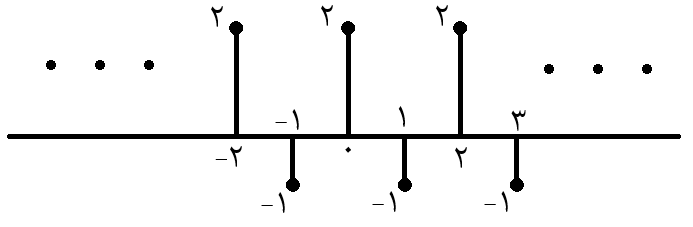
\includegraphics[width=65mm]{m3}
\end{center}
از سیستمی با پاسخ فرکانسی زیر عبور کند
\begin{center}
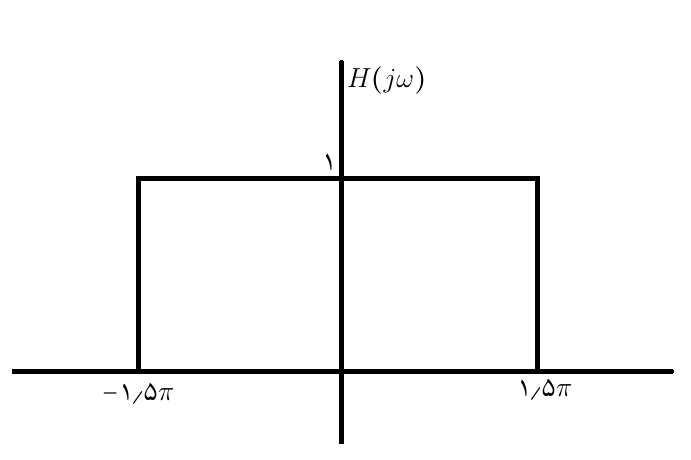
\includegraphics[width=65mm]{m4}
\end{center}
خروجی را بیابید.




(می توانید سایر اصلاحیات را در اینجا اعمال فرمایید)









}





\end{RTL}



\end{document}


